 
\renewcommand\chapname{Deconstructing descriptive grammars}	
\renewcommand\longchapname{Deconstructing descriptive grammars}
\renewcommand\shortauthor{Jeff Good}
\renewcommand\longauthor{Jeff Good

 University of Buffalo}
\chapter*{\longchapname}
\chapterauthor{\longauthor}
\mytoc{}

 


% \parbox{5in}{\small \noindent
% \section{Abstract}
\begin{abstract}
Much work within digital linguistics has focused on the problem of developing
concrete methods and general principles for encoding data structures designed
for non-digital media into digital formats. This work has been successful enough
that the field is now in a position to move past ``retrofitting'' digital
solutions onto analog structures and to consider how new technologies should
actually change linguistic practice. The domain of grammaticography is looked at
from this perspective, and a traditional descriptive grammar is reconceptualized
as a database of linked data, in principle curated from distinct sources. Among
the consequences of such a reconceptualization is the potential loss of two
valued features of traditional descriptive grammars, here termed \emph{coverage}
and \emph{coherence}. The nature of these features is examined in order to
determine how they can be integrated into a linked data model of digital
descriptive grammars, thereby allowing us to benefit from new technology without
losing important features intrinsic to the structure of the traditional version
of the resource.
\end{abstract}
% 
% \bigskip

%%%%%%%%%%%%%%%%%%%%%%%%%%%%%%%%%%%%%%%%%%%%%%%%%%%%%%%%%%%%%%%%%%%%%%%%%%%%%%%%
\section{From recoding to reconceptualizing\label{Intro}}
%%%%%%%%%%%%%%%%%%%%%%%%%%%%%%%%%%%%%%%%%%%%%%%%%%%%%%%%%%%%%%%%%%%%%%%%%%%%%%%%

The field of linguistics is now well aware of the need to use new digital
technologies to encode linguistic data with care in order to ensure its
portability across user communities, computational environments, and even time
\citep{Bir:Sim:03}.\footnote{I
 would like to thank audience members at the Colloquium on Electronic Grammaticography,
 held at the Second International Conference on Language Documentation and Conservation
 at the University of Hawai`i at M\=anoa, February 11--13, 2011, as well an anonymous
 reviewer, for their comments on the work leading to this paper.
 Many of the ideas developed here have been influenced by informal discussions
 with a number of individuals during the last several years,
 in particular Michael Cysouw and Sebastian Nordhoff.}
This has resulted in a
range of work examining the best means through which traditional linguistic
resources can be re-encoded in digital form. Proposals have been made, for
instance, that offer conceptual models and accompanying digital implementations
for lexical resources \citep{BellBird:2000,PoornimaGood:2010}, interlinear
glossed text \citep{BBB:2003,SchroeterThieberger:2006,PalmerErk:2007},
grammatical paradigms \citep{PentonEtAl:2004}, and descriptive grammars
\citep{Good:2004Metadatabase} (see also \citet{Drudetv} and \citet{Thiebergertv}). Other work has gone beyond this to codify general
principles for conducting this kind of research, as seen, for instance, in
\quotecite{Nordhoff:2009} examination of possible ideal requirements for
electronic grammars and in the ``meta-model'' approach to lexical encoding
embodied by Lexical Markup Framework, developed in the context of work on
natural language processing \citep{Francopoulo:2009} (see also
\namecite{WittenburgEtAl:2002} and \namecite{Trippel:2006,Trippel:2009}).

This work has produced important results, and, in particular, has made clear
that, even if important kinds of linguistic data may still await proper study,
the challenges of encoding them linguistically are presumably solvable using
existing technologies, in particular generalized markup systems like XML (see
\namecite[225--227]{Good:CUPHEL} for discussion of XML in the context of
language documentation). Furthermore, it is even possible to extract from this
body of research an informal general procedure for devising new encoding
schemes: (i)~survey existing practice for presenting data in a given domain,
(ii)~devise a conceptual model of the data that can be understood as providing
an underlying form for the surveyed presentation (or ``surface'') forms,
(iii)~relate the various components of that model to linguistic practice,
focusing, in particular, on how they can be derived from more general principles
regarding what constitutes appropriate  methodology for linguistic analysis, and
(iv)~propose a concrete way of encoding that model using archival markup formats
that is as consistent with those general methodological principles as possible.
While I am not aware of any one publication that incorporates the totality of
these procedures, the combination of \namecite{Good:2004Metadatabase} and
\namecite{Nordhoff:2009} can be understood as an illustration of this approach
in the domain of descriptive grammars (see also \citet{Nordhofftv}).

At the same time, the sensible reliance of such work on \emph{existing} practice
makes it ill-suited for considering the ways in which new technologies should
prompt more fundamental reconceptualizations of the kinds of products that the
field of linguistics should produce as a result of technological changes. This
is illustrated, for instance, by \quotecite{PalmerErk:2007} revision to
\quotecite{BBB:2003} proposals for encoding interlinear glossed text. The
latter is sufficient for dealing with interlinear glossed text's traditional
function of providing a succinct analysis of the lexical and grammatical content
of a given stretch of phrasal data. However, it is not well-suited for an
additional function that is clearly desirable (though non-traditional):
automated (or semi-automated) annotation.

The main goal of this paper is to consider how new models for data
encoding---developed independently from the field of linguistics---might prompt
us to consider revisions to our models for producing traditional grammatical
descriptions. In particular, detailed consideration will be given regarding how
the work required to describe a language's grammar on the basis of documentary
products might be done in a highly distributed fashion by making use of emerging
Web technologies (sections \ref{Context} and \ref{Facets}). However, as we will
see, there is a danger when considering such a possibility: The introduction of
a new conceptualization of a linguistic resource, with clear positive features,
may inadvertently lead to the loss of valued features embedded within
traditional models. This requires the development of means to reintegrate what
has been ``lost'' into the new conceptualization, which can be done by
augmenting received technologies with solutions more specific to linguistics
(sections \ref{Coverage} and \ref{Coherence}). However, the solutions discussed
here only allow us to retain part of what would be lost, underscoring that the
transition from traditional products to digital ones must be led by linguists'
needs rather than the non-linguistic agendas that drive the development of most
new technologies (\sref{Conclusion}).

This paper is primarily conceptual in nature, rather than reporting on the
results of a specific technological implementation. Accordingly, at times, it
will be somewhat speculative, though an attempt will be made, whenever possible,
to ground any speculation in relevant existing technological efforts, often from
within linguistics itself. The intended audience for this paper are so-called
ordinary working linguists, rather than those more directly engaged in applying
emerging technologies to linguistic work. At the same time, I hope that some of
its key ideas will be of interest to both groups. Those familiar with work on
the technologies to be discussed will be aware of the fact that some of the
points made here are relatively well-known outside of linguistics. Therefore, in
some places, the aim of the discussion will not be to outline the significance
of these new technologies generally but, rather, to present them in a way that
makes their utility clearer to a documentary and descriptive linguistic
audience---that is, to linguists who are now, or may in the future, be creating
new grammatical descriptions.



%%%%%%%%%%%%%%%%%%%%%%%%%%%%%%%%%%%%%%%%%%%%%%%%%%%%%%%%%%%%%%%%%%%%%%%%%%%%%%%%
\section{The technological context\label{Context}}
%%%%%%%%%%%%%%%%%%%%%%%%%%%%%%%%%%%%%%%%%%%%%%%%%%%%%%%%%%%%%%%%%%%%%%%%%%%%%%%%

While some data encoding technologies (e.g., XML) have become so ubiquitous in
work on language documentation and description as to require little
introduction, the technological context which inspires the present work---that
of the so-called Semantic Web---has not yet been particularly widely employed
within linguistics. The leading idea behind the development of the Semantic Web
is to extend the document-centered World Wide Web to all kinds of data, adding,
in effect, an explicit layer of meaning to a network architecture that was
originally designed to simply link together pages intended to be interpreted by
humans.{\footnote{The Semantic Web Frequently Asked Questions page
({http://www.w3.org/2001/sw/SW-FAQ}) produced by the World Wide Web Consortium
serves as useful introduction to the Semantic Web. See also
\namecite[2--5]{ChiarcosEtAlIntro:2012} and \namecite[129--131]{Moran:2012}
for additional introductory discussions in a linguistic context.}}

Rather than consisting of a monolithic piece of technology, the Semantic Web is
better understood as resulting from the interactions of a set of
logically-independent technological pieces. Some of these are relatively simple
in and of themselves but, nevertheless, provide crucial elements of the
infrastructure needed to augment the World Wide Web with semantic information.
Moreover, since the Semantic Web is intended to build on the World Wide Web,
many of its core technologies are the same as those of the World Wide Web
itself, as seen, for example, in its use of Unicode for character encoding (see,
e.g., \namecite{Anderson:EMELD:2003} and \namecite[345--351]{Gippert:2006} for
discussion of Unicode in a linguistic context). At the same time, in order to
extend the World Wide Web, there are also technologies that underlie the
Semantic Web that are not part of the World Wide Web. The most prominent of
these within work on language documentation and description is almost certainly
Web Ontology Language (OWL), which has been used to express the linguistic
information encoded in the General Ontology for Linguistic Description (GOLD)
\citep{FarrarLangendoen:2003,FarrarLewis:2007,FarrarLangendoen:2009}.{\footnote{The
latest version of GOLD can be viewed at http://linguistics-ontology.org/.}}
GOLD will be returned to shortly below.

The Semantic Web technologies that will play a significant role in the
discussion here are given in \tref{SWTech}. (The first of these, the URI, is
also a World Wide Web technology and likely to be familiar to many readers.) A
brief summary of the relevant function that each takes on is included in the
table, though this description should not be understood to be exhaustive in a
general Semantic Web context. Both in the table, and elsewhere, the presentation
of the Semantic Web and relevant component technologies is simplified somewhat
for the purposes of exposition.

\begin{table}[ht]
\centering
\begin{tabular}{@{}lll@{}}
\Hline
{\sc acronym}	&	{\sc technology}				&	{\sc function}		\\
\Hline
URI				&	Uniform Resource Identifier		&	Unique identification of entities	\\
RDF				&	Resource Description Framework	&	Description of entities				\\
OWL				&	Web Ontology Language 			&	Encoding of general facts 			\\
\Hline
\end{tabular}
\caption{Some Semantic Web Technologies \label{SWTech}} 
\end{table}

Taken together the three technologies listed in \tref{SWTech} allow for (i)~the
unique reference to anything in the real or mental world (e.g., a language, an
utterance, or a phoneme) in the form of URIs, (ii)~the specification of
``facts'' about those entities (e.g., \emph{English is a language} or \emph{this
sentence makes use of a passive construction}) in the form of RDF expressions,
and (iii) the specification of the overall properties of the conceptual model
that the entities and facts are embedded within (e.g., \emph{sentences have
grammatical properties} or \emph{lexical items are comprised of a combination of
sound, meaning, and grammatical properties}) in the form of OWL statements.
While the ability to specify such information falls short of the rich content of
a traditional descriptive grammar, it should be clear
that even this relatively minimal apparatus could allow for the production of a
significant amount of description of a given language's grammar. In particular,
it would permit many of the ``low-level'' facts that are part of any complete
grammatical description to be encoded in a machine-readable form on the Web.

It would be inappropriate to cover the full technical details of URIs, RDF, or
OWL here. However, it will be useful if something can be said about what these
technologies ``look like'' in concrete terms, especially since none of them is a
prototypical instance of a ``technology''. In Semantic Web applications, URIs
look more or less like the familiar Uniform Resource Locators (URLs) associated
with web pages, taking on a form like \texttt{http://example.org/English}. URLs can, in
fact, be understood as a type of URI that both identifies a given entity (e.g.,
a web page or a file) and also specifies how the entity can be found on the
World Wide Web. While Semantic Web URIs look like URLs, and may even behave like
URLs in resolving to a web page when accessed on a browser, strictly speaking
they need not be URLs. In concrete terms, this would mean that if a URI, which
was not also a URL, were entered into a browser, it would not resolve to any web
page (and produce, for example, an error page).

The idea that a URI may look like URL, but not act like one, is potentially
counterintuitive to those accustomed to working with the World Wide Web rather
than the Semantic Web. However, it is a reasonable consequence of attempting to
build an online repository of information on top of the existing Web rather than
in a completely new environment. In this case, the standard Web mechanism for
uniquely referring to a given web page is simply extended for uniquely referring
to \emph{anything}, whether or not it happens to be associated with a web page.
Of course, alternatives are possible. For instance, the Handle System provides
another mechanism for creating unique identifiers (see
\namecite{BroederEtAl:2006} for discussion of the use of the Handle System in
developing linguistic infrastructure).{\footnote{The Handle System is used by
this journal as a means of persistent identification for published papers. For
example, the handle for \namecite{Newman:2007} is 10125/1724. This handle can be
resolved, using an appropriate online service, to a web page where a copy of the
paper can be found. One way to do this is to simply append the handle to
http://hdl.handle.net/, producing the URL http://hdl.handle.net/10125/1724.}}

An important feature of URIs is that they are not merely unique within some
local system, as might be the case, for instance, for identification numbers of
the sort commonly associated with records in a database. Rather, they are
universally unique in the context of the Web, at least when used as intended.
That is, in Semantic Web terms, anything that needs to be referred to gets a
completely unique identifier. The vast proliferation of identifiers that this
entails may, at first, sound problematic. However, one must bear in mind
that the World Wide Web has grown vastly since its first inception without
breaking down, illustrating the durability of URIs as a mechanism for
providing globally unique references.

Turning now to the second technology listed in \tref{SWTech}, Resource
Description Framework (RDF) is a means for making machine-readable three-part
statements, or \emph{triples}, of the form {\sc {subject~predicate~object}}.
The subject is a URI for some entity, the predicate is a URI for a possible
relationship between a subject and an object, and the object consists of either
of a URI or a limited class other objects, such as a text string. Figure
\ref{RDFExample} gives an example of a representation of two RDF triples. The
first (Triple 1) is intended to relate a subject URI referring to the English
language to an object URI referring to the phoneme \emph{p} via a predicate that
states that that phoneme is found in English (i.e., ``English has the phoneme
\emph{p}''). The second (Triple 2) relates the phoneme \emph{p}, now serving as
a subject of a triple, to its standard transcription, the text string ``p'',
serving as the object of the triple (i.e, ``The phoneme \emph{p} has the
transcription `p''').



\begin{figure}[ht]
\centering
\scalebox{.5}{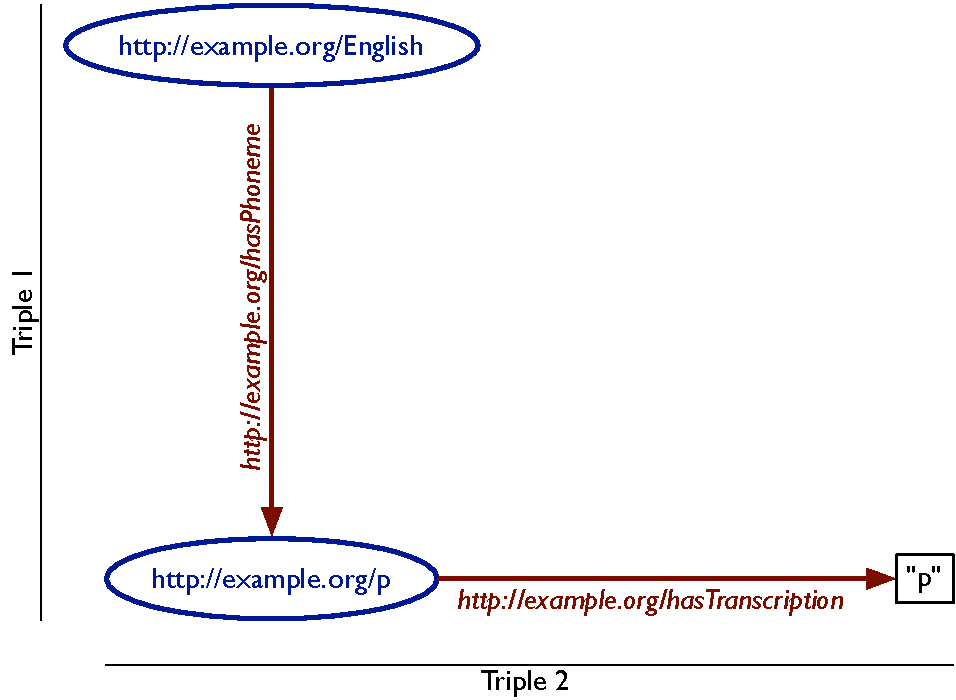
\includegraphics{\imgpath/RDFTriples.pdf}}
\caption{Two RDF triples }
\label{RDFExample}
\end{figure}

RDF has not yet been widely deployed for describing traditional linguistic data,
though there have been some attempts, both as exemplary cases \citep{Simons:2005}
and in working systems \citep{GoodParker:2006} (see also
\namecite[63--65]{Cysouw:2007:Social}).{\footnote{The websites for the World
Atlas of Language Structures (WALS) \citep{WALS:2011}, the World Loanword
Database \citep{WOLD}, and Glottolog/Langdoc \citep{Nordhoff:2012} all allow
data to be exported in RDF format,
though in the case of WALS, this is limited to bibliographical data.}} It has
also seen attention in research in computational linguistics (see, e.g.,
\namecite{IdeEtAl:2003}).

The information encoding model of RDF is, in principle, expressible in a variety
of formats, including a standardized XML format, which facilitates exchange of
data described in RDF. More generally, RDF can be understood as a means for
encoding data that can usefully be modeled in the form of a graph consisting of
nodes connected by labeled arcs, as is seen in \fref{RDFExample}.{\footnote{The
fact that the connections between nodes in RDF representations can be labeled or
``typed'' makes them richer than the connections found in typical hypertext
which merely links documents (or parts of documents) without specifying the
semantic nature of those links. Therefore, while ``hypertext grammars''
\citep[29]{EvansDench:2006} would clearly represent an advance over traditional
grammars, they would fall short of the possibilities afforded by the Semantic
Web.}} Of course, RDF is not the only way of describing data in graph form,
though it is the focus here because of its role as a key means of expressing
``atomic'' statements about entities in the context of the Semantic
Web.{\footnote{Another common way of expressing graphs with labeled arcs in
linguistic work is through the use of feature structures as found, for example,
in Head-driven Phrase Structure Grammar \citep[50--51]{SWB:2003}.}}

An important feature of graphs (whether or not they are expressed in RDF) is
that, as discussed by \namecite{IdeSuderman:2007}, they facilitate the merging
of information from distinct sources. As long as two related sets of data
expressed in graph form use the same identifiers for nodes referring to the same
entities, the two graphs can simply be joined wherever nodes are shared. If we
consider \fref{SWTech}, for instance, one data source could state that English
makes use of the phoneme \emph{p}, while another could associate \emph{p} with a
transcription, with the two being joined by their common node,
http://example.org/p. While this is a relatively trivial example, graph merger
of this kind can become quite powerful when the merged graphs each contain rich
and largely complementary information (see \sref{Disentangling}).

URIs and RDF, when brought together, are key pieces to the idea of creating
significant amounts of \emph{Linked Data}, which is seen as a crucial step
towards the broader vision of the Semantic Web \citep[15]{BizerEtAl:2009}
and provides a useful metaphor for understanding the goals of the Semantic
Web more generally.{\footnote{A workshop on Linked Data in Linguistics was
held on March 7-9, 2012, in Frankfurt, Germany (see http://ldl2012.lod2.eu/)
and resulted in an edited volume \citep{LDL:2012}.}}

The final technology listed in \tref{SWTech} is Web Ontology Language (OWL),
which allows for the expression of \emph{ontologies}. In this context an
ontology can be understood as a means for expressing general knowledge about a
given domain in a form that can be understood by machines. This might include
statements like, \emph{a past tense is a kind of tense} or \emph{a phoneme
inventory is comprised of phonemes}. Basic statements like these could, in fact,
be stated using RDF which is flexible enough to encode both very specific
statements as well as general ones. OWL, however, provides a means for
expressing certain kinds of generalizations that are not standardly expressible
in RDF. In fact, OWL can itself be viewed as an augmentation of RDF in much the
same way as the Semantic Web augments the World Wide Web. To pick one example,
OWL provides a standard way of stating that one property is the ``inverse'' of
another property. This would allow, for instance, a machine to infer that, if
\emph{the phoneme \emph{p} has the transcription `p'}, then \emph{the symbol
`{p}' is a possible transcription of the phoneme \emph{p}}. As discussed above,
there has already been significant work on an OWL-based ontology in the context
of descriptive linguistics in the form of the GOLD project
\citep{FarrarLangendoen:2003,FarrarLewis:2007,FarrarLangendoen:2009}, and there
has also been work using OWL to support the mobilization of descriptive language
materials \citep{BeckEtAl:2007}.

Before moving on, it is important to bear in mind that URIs, RDF, and OWL are
merely specific technical solutions to more general problems. Their significance
in the present context is the way that they are integrated into the larger
vision of the Semantic Web. Of course, the Semantic Web, too, is a specific
technical solution to the broad problem of how information can be shared and
exchanged efficiently. Its relevance for the field of linguistics is twofold.
First, it offers a model for a new way of managing research results in an
increasingly internet-driven data management world. Second, it is a specific
instantiation of such a model with considerable support outside of linguistics,
allowing linguists to take advantage of technological infrastructure that has
already been developed elsewhere.

The next section of this paper will consider how an initiative like the Semantic
Web might prompt us to reconsider what it means to create a descriptive grammar
of a language.




%%%%%%%%%%%%%%%%%%%%%%%%%%%%%%%%%%%%%%%%%%%%%%%%%%%%%%%%%%%%%%%%%%%%%%%%%%%%%%%%
\section{Multiple facets of grammars\label{Facets}}
%%%%%%%%%%%%%%%%%%%%%%%%%%%%%%%%%%%%%%%%%%%%%%%%%%%%%%%%%%%%%%%%%%%%%%%%%%%%%%%%

%%%%%%%%%%%%%%%%%%%%%%%%%%%%%%%%%%%%%%%%%%%%%%%%%%%%%%%%%%%%%
\subsection{Disentangling publication\label{Disentangling}}
%%%%%%%%%%%%%%%%%%%%%%%%%%%%%%%%%%%%%%%%%%%%%%%%%%%%%%%%%%%%%

In this section, I will largely abstract away from the technical details
delineated in \sref{Context} and, instead, focus on how the model embodied by
the conjunction of the technologies in \tref{SWTech} could be exploited to
create new methods for producing grammatical descriptions. In principle, a
number of the ideas developed here could have been put forth decades ago. After
all, many of the key concepts embodied by the Semantic Web (e.g., unique
identification) are hardly new. However, in practice, before the rise of the
World Wide Web, work along such lines would have been largely impossible to
apply concretely to documentary and descriptive research. We have now reached a
point, by contrast, where the development of models that, at one point, would
have been merely speculative or ``futuristic'' can actually be implemented in
specific tools, at least in prototype form. This makes it important for the
field to begin to consider the relevant issues proactively in order to avoid
accidentally adopting technological solutions that might, at first, appear to be
appropriate but which may actually be built on assumptions that will prove
problematic in the long run. (See \namecite[134--138]{BoyntonEtAl:2010} for
relevant discussion in a language documentation context.)

A striking feature of the model that the Semantic Web
offers is the extent to which it leads to a view of scholarly work in
general, and grammaticography more specifically, wherein a number of elements
that were previously intertwined due to the restrictions of paper
publication can now be decoupled from one another. Based on ideas found in
\namecite{Neylon:2010}, we can break down the functions of traditional
``monolithic'' scholarly publications along the lines of what is described
in the following list.


\begin{enumerate}
\label{Publishing}

	\item{{\bf Registering:} Scholarly publishing allows an individual or
	set of individuals to officially establish that they should be associated
	with a given set of ideas or research results. \label{Registering}}
	
	\item{{\bf Filtering:} Scholarly publishing provides mechanisms through
	which a given user can locate the information they are interested in
	both by providing a means through which the quality of a given piece of
	research can be quickly
	assessed and by providing tools for discovery (e.g., through the use of
	keywords).}

	\item{{\bf Curation:} Scholarly publishing works with carefully aggregated
	sets of data that are brought together to tell a specific ``story''.
	\label{Curation}}
	
	\item{{\bf Archiving:} Scholarly publishing produces resources designed to
	be usable in the long-term.}
	
	\item{{\bf Reusing:} Scholarly publishing is associated with standardized
	mechanisms through which research results can be reused in a manner deemed
	acceptable by the research community (e.g., by providing a stable
	citation for a given resource).}

\end{enumerate}
	

Of the five functions of publishing given above, the one of
greatest interest here---and the one which would would seem to be most
profoundly impacted by the technologies discussed in \sref{Context}---is almost
certainly the curatorial function. The traditional model of a
descriptive grammar as a kind of monograph encourages us to see the thousands of
tiny observations that form a complete description as part
of a single research ``outcome''. The graph-based model of the Semantic Web, by
contrast, explicitly makes each of these observations visible as distinctive
connections among discrete objects. This was already schematized in
\fref{RDFExample}, with a relatively simplistic example. Figure \ref{Analysis}
offers something comparable with a more complex example that abstracts away from
some of the more technical aspects of RDF.

\begin{figure}[ht]
\centering
\scalebox{.5}{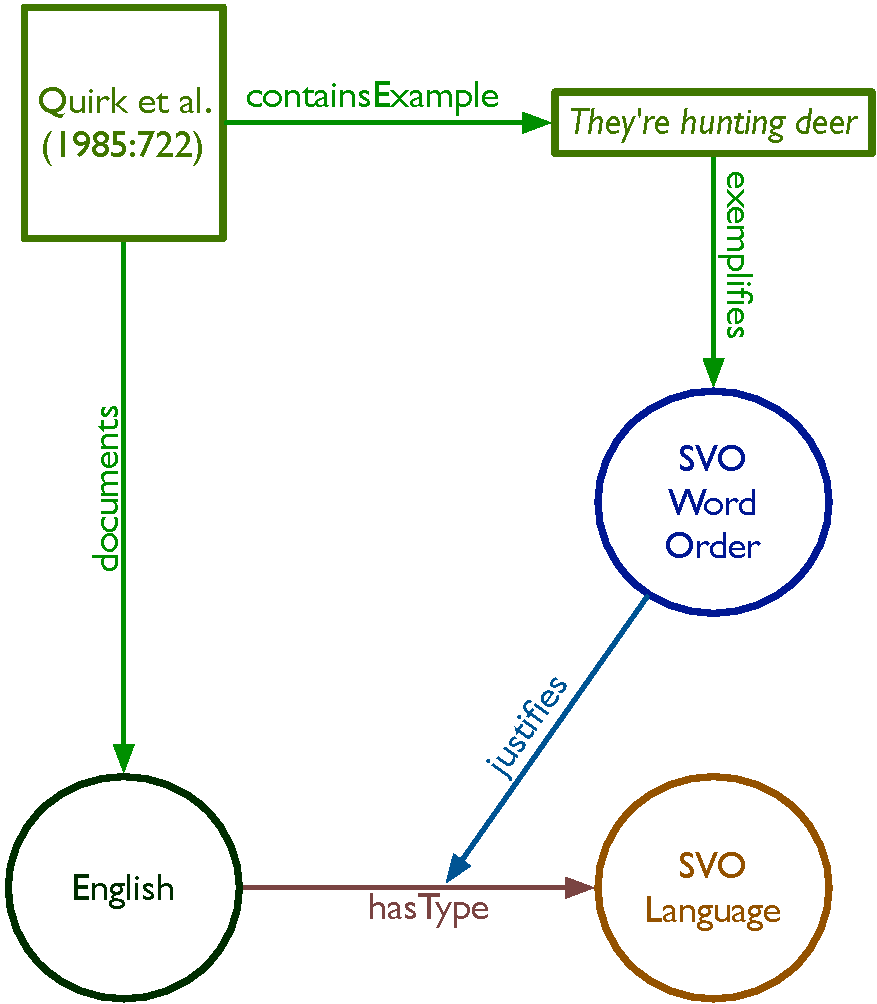
\includegraphics{\imgpath/Analysis.pdf}}
\caption{A fragment of a descriptive grammar in graph form \label{Analysis}}
\end{figure}

\nocite{QuirkEtAl:1985}

Figure \ref{Analysis} represents a set of low-level statements which, when
combined, allow one to make a claim like \emph{English is an SVO language}. At
the top of the figure, an example is indicated as being extracted from a source
that documents the English language. This example is observed to show SVO word
order, which, in turn, justifies the general classification of English as an SVO
language. In RDF terms, this would mean breaking down the classification of
English as SVO into five distinct statements (or triples). There are obvious
elements of simplification involved in the figure, though it should be
sufficient for purposes of exemplification.

By way of further illustration, figure \ref{Genealogy} represents further
information about one of the nodes in \fref{Analysis}, the one representing the
English language. This figure gives reference information for English,
specifically a language code and its genealogical parent. It can be understood
here as representing information about the same entity as described in
\fref{Analysis}, but coming from a different source.

\begin{figure}[ht]
\centering
\scalebox{.5}{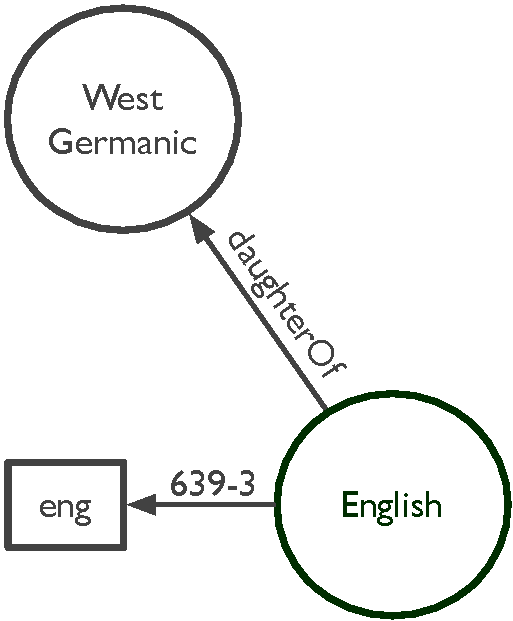
\includegraphics{\imgpath/Genealogy.pdf}}
\caption{Classificatory information for English in graph form \label{Genealogy}}
\end{figure}

Figure \ref{Merger} illustrates one of the positive features of graph-based
representations of information (see also \sref{Context}): The fact that they
allow information from different sources to be straightforwardly merged as
long as common node identifiers are employed. In \fref{Merger}, the content
of figures \ref{Analysis} and \ref{Genealogy} are brought together into a single
graph.

\begin{figure}[ht]
\centering
\scalebox{.42}{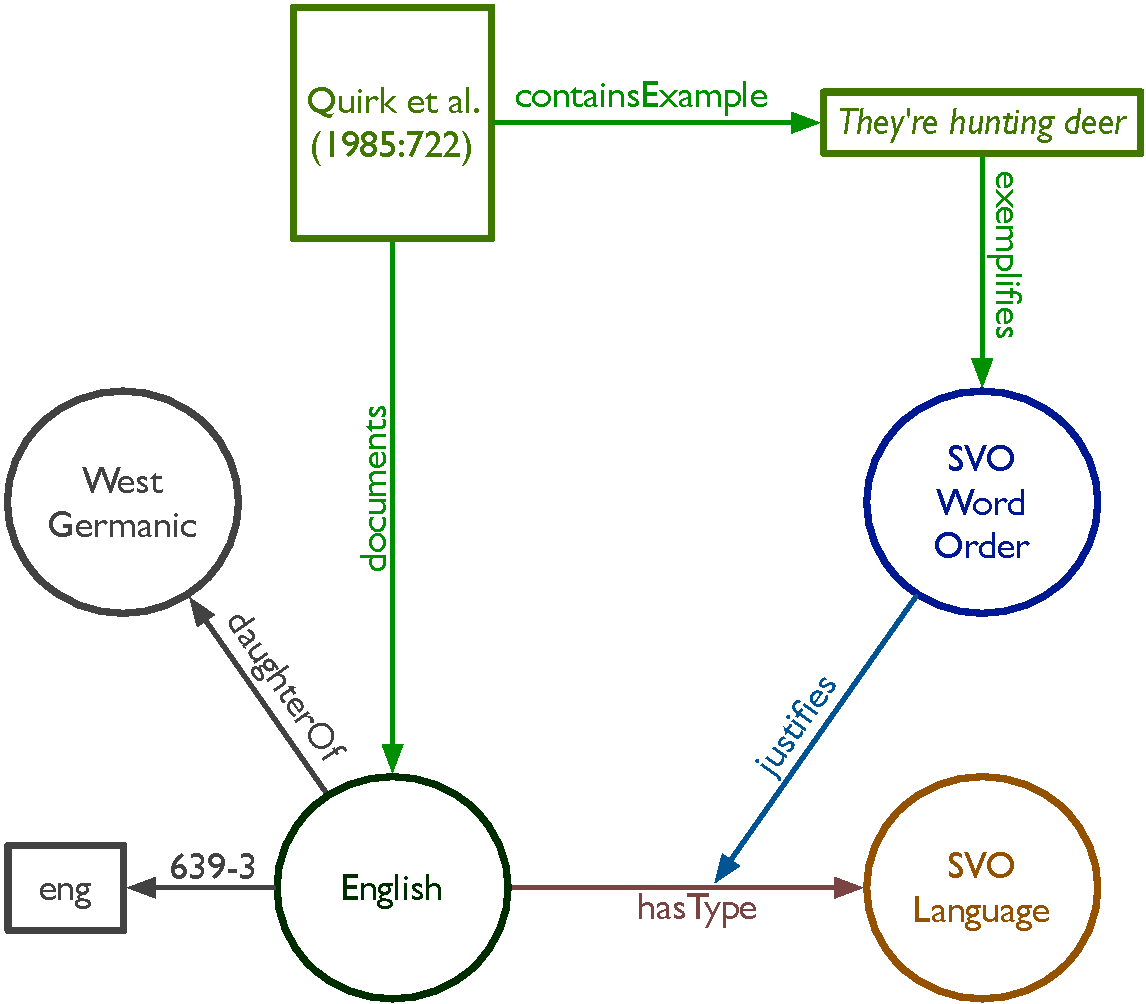
\includegraphics{\imgpath/Merger.pdf}}
\caption{Merging two graphs \label{Merger}}
\end{figure}

Of course, there is nothing particularly innovative about combining related
pieces of information from distinct sources. The power of graph-based
representations like the one seen in \fref{Merger} is the way in which they
allow this process to be, at least partly, automated and the way in which they
make visible the nature of the connections between data sources in a more
precise way than is possible with standard academic citations.

This latter point is of interest here when we consider the inherently
``distributed'' task of writing a descriptive grammar---even if it is only
written by a single author. They are typically the distillation of a number of
years, or even decades, of work on a language and untold numbers of small
observations, preliminary analyses, reanalyses, etc. (see
\namecite[417--418]{Weber:2006} for relevant discussion). Moreover, the
distributed nature of the work involved in grammar writing has become
significantly more pronounced in recent years with the rise of the documentary
paradigm. This has stressed methodological and theoretical separation between
research outputs that can be classified as ``documentary'' from those that are
``descriptive'' (\citeboth{Himmelmann:1998};
\citeboth[168--169]{Woodbury:2011}). The next section will consider then what a
``graph-based'' approach to data might mean for grammar writing, especially in
the context of the newly placed emphasis on documentation. A more concrete way
of looking at this issue would be to ask: How would grammar creation be
different if crafting each of the component statements of a classification like
the one represented in \fref{Analysis} was the responsibility of different
linguists?

Before moving on, it seems worth emphasizing that many of the issues to be
addressed below---for example, ensuring that a grammar has adequate coverage or
that its analyses are coherent---existed long before the development of digital
approaches to research. What has changed is that, now that research can, in
principle, be done in a much more distributed fashion, the utility of general
solutions to problems like these has become more apparent. In the creation of
single-authored grammars, the main control on coherence, for example, has been
the authors themselves. But clearly this concern must be approached differently
if one wants to make use of the time and the skills of ten, or even a hundred,
contributors working on the description of a single language. Moreover, as we
will see in the next section, there has been impetus for grammatical
descriptions to be developed in a more distributed fashion that has arisen
completely independently from the growth of the Semantic Web itself.


%%%%%%%%%%%%%%%%%%%%%%%%%%%%%%%%%%%%%%%%%%%%%%%%%%%%%%%%%%%%%
\subsection{Towards distributed grammar authoring\label{Authoring}}
%%%%%%%%%%%%%%%%%%%%%%%%%%%%%%%%%%%%%%%%%%%%%%%%%%%%%%%%%%%%%

The extent to which the activities comprising documentation and description
should be viewed as easily severable has been questioned (see, e.g,
\namecite[346--348]{Evans:2008}). Nevertheless, it seems uncontroversial that
the possibilities that new technologies offer for creating documentary products
should have a significant impact on the creation of grammatical descriptions
(\citet[24--25]{EvansDench:2006}, see also \citet[120--122]{Good:LDPV}).
Moreover, the documentary paradigm has emphasized the need for a more
collaborative approach to the collection and analysis of language data,
integrating members of speaker communities, as well as experts from allied
disciplines, more directly into the linguist's research activities
(\citeboth[15--16]{Himmelmann:2006}; \citeboth[54--55]{Dwyer:2006};
\citeboth[293--399]{Grenoble:2010}; \citeboth[176--177]{Woodbury:2011}).

While not always emanating from the same fundamental concerns, both of these
ideas share a comparable impact when it comes to research which has as one of
its goals the production of a descriptive grammar. On the one hand, new data
collection and annotation technologies have led to an emphasis on ensuring that
the provenance of a descriptive claim can be straightforwardly verified by
associating it with the relevant supporting documentary materials. Ideally,
these should be in the form of fully transcribed texts as well as audio and
video records (see, e.g., \namecite[571]{Bir:Sim:03};
\namecite[299]{Nordhoff:2009}; \namecite{Thieberger:2009}). This requires tools
and methods for making the ``documentary chain'' from recording to analysis
explicit, which amounts to creating a new set of intermediate linguistic
resources comprising each of the relevant links in that chain. A prominent
example of this is time-aligned annotation, which connects a transcription
directly to the recording containing what is being transcribed. This has
resulted in the widespread use of a relatively new kind of linguistic resource
which encodes documentary and descriptive annotations (see
\namecite{SchultzeBerndt:2006} and \citet{Boudatv}) directly with an indication of start and end
times within a media file that those annotations can be associated with. This is
found, for example, in resources produced by the ELAN annotation tool (see
\namecite{Berez:2007} for a review). What we see in this case is that the task
of annotation, which formerly was disseminated primarily as embedded within
finished products, can now be associated with an ``intermediate'' resource
reflecting an important aspect of the underlying work.{\footnote{Of course,
``intermediate'' objects like this could be created without the aid of new
digital technologies and some of them can be found in archives of field notes.
However, before the rise of the internet, they were not typically made widely
available or as carefully curated.}}

On the other hand, collaborative models for collecting and analyzing linguistic
data cause us to shift perspective from an approach where a single individual is
responsible for all stages of grammatical analysis to one where the various
stages of the documentary and descriptive workflow might be the primary
responsibility of different contributors (see, e.g., \namecite{Thieberger:2004}
and \namecite[461--462]{Bowern:2011} for discussions of workflow). This adds an
additional element of ``decomposition'' to the traditional way of working. In
large part, new data management and communication technologies are a
prerequisite to the practical application of such collaborative models. However,
their ultimate motivation is largely social in nature and emanates from changes
in the conception of what constitutes ethical and appropriate research practices
(see, e.g., \namecite[124--134]{Rice:2006} and
\namecite[201--206]{DobrinBerson:2011}). They can also be understood as a
response to language endangerment, insofar as the impending loss of a language
is understood as a loss not only to linguistics, but to speaker communities and
other disciplines as well. This has, thereby, caused linguists to seriously
consider the need for approaches incorporating a diverse array of stakeholders
in the collection and analysis of language data. Here, then, we see how a set of
changes in practice, driven by social considerations, can at least be partly
supported by new technologies---in this case, technologies which facilitate work
being done in distributed fashion.

Taken together, these two trends place increasing emphasis on the individual
``pieces'' of work involved in the creation of descriptive grammars, as opposed
to treating them as a monolithic whole---the view encouraged by the traditional
publication model. Moreover, independent of developments within work on language
documentation itself, a more distributed approach to work forming the basis of
descriptive grammars, in principle, has an additional potential advantage: It
can facilitate more efficient use of research resources. An individual who is
skilled at transcription may not be adept at morphological analysis, and a
specialist in semantics may not be the ideal person to work on a language's
phonemic system---and this is not to mention the problems that may arise when a
linguist is asked to be not merely a grammarian but also an archivist,
ethnographer, a lexicographer, or even a ``linguistic social worker''
(\citet[14--17]{Newman:1998}, see also \citet[342--343]{Evans:2008}).

We arrive then, at a potential future where we move away from the
publication-centered view of a descriptive grammar as a single-authored
monograph to one where it consists of the compilation of set of ``facts'' about
a language, each associated with a distinct provenance. This view of a
``grammar'' not only has clear connections to the current documentary paradigm,
but it is also consonant with the reconceptualization of data embodied by the
Semantic Web: Research results are ``atomized'' as it were, the barriers to
registering a result (in the sense of developed in \sref{Disentangling}) are significantly
reduced, and the connections between discrete results can be made more explicit.
Of course, it is a long road from the representation of a relatively simple
observation like that seen in \fref{Analysis} to the construction of a graph
representing a ``complete'' descriptive grammar. Nevertheless, we now have a
core conceptual model of such a structure, technology that can implement that
model, and even a field-internal motivation to use such a model. This
means the creation of such an object is no longer simply something only
to be imagined.

Within this broad vision, making the results of research public no longer needs
to be delayed until it reaches the threshold of a ``publishable unit'' (see
\namecite{Broad:1981}) but can be done as soon as a useful observation is made,
even if it constitutes something as simple as the discovery of a new minimal
pair or a single unusual pattern of agreement. Of course, such
``micro-discoveries'' would not be associated with the same level of prestige as
a curated publication.{\footnote{The idea of publishing a ``micro-discovery''
can be clearly connected to the notion of micro-blogging, most prominently
associated at present with the online service Twitter (http://twitter.com),
which has been the subject of work considering how the content of micro-blogs
can be made available not just on the World Wide Web but within the Semantic Web
as well \citep{PassantEtAl:2010}. See also \namecite[64]{Cysouw:2007:Social} for
relevant discussion on the notion of a ``micro-publication'' within work on
language typology.}} What is important is that the Semantic Web, in principle,
can allow them to be associated with the elements of publishing appropriate to
them, e.g., registration, archiving, and reuse (see \sref{Disentangling}), even if
they fall short of the whole traditional publication ``package''.

There are clear potential advantages to reconceptualizing descriptive grammars
as distributed, multi-authored resources. However, it is immediately apparent
that valued features of the traditional descriptive grammar would be lost under
such an approach unless additional measures are taken. In particular, the
curatorial aspect of publishing (see \sref{Disentangling}) imposes various important
characteristics on the assembled ``facts'' which constitute descriptive
grammars, two of which I will focus on here, \emph{coverage} (\sref{Coverage})
and \emph{coherence} (\sref{Coherence}). Of course, these are only parts of what
constitutes a ``good'' grammar (see, e.g.,
\namecite{Noonan:2006,Rice:2006:Grammars}), an issue which will be briefly
returned to in \sref{Deconstructing}.




%%%%%%%%%%%%%%%%%%%%%%%%%%%%%%%%%%%%%%%%%%%%%%%%%%%%%%%%%%%%%
\section{Coverage \label{Coverage}}
%%%%%%%%%%%%%%%%%%%%%%%%%%%%%%%%%%%%%%%%%%%%%%%%%%%%%%%%%%%%%

%%%%%%%%%%%%%%%%%%%%%%%%%%%%%%%%%%%%%%%%%%%%%%%%%%%%%%%%%%%%%
\subsection{Coextensivity and completeness\label{TwoCoverages}}
%%%%%%%%%%%%%%%%%%%%%%%%%%%%%%%%%%%%%%%%%%%%%%%%%%%%%%%%%%%%%

An important aspect of good descriptive grammars is the extent to which their
discussion (i) adequately addresses phenomena represented in the available
documentation on a language and (ii) presents a reasonable overview of a
language's entire grammatical system.{\footnote{By \emph{available
documentation}, I refer to the extent of the documentary resources (e.g.,
recordings, transcribed texts, lexical material, etc.) that those working on the
description of a given language have access to when doing their work.}} I refer
to these properties under the umbrella term \emph{coverage} here, using the term
\emph{coextensivity} for the relationship between a description and available
documentation and \emph{completeness}, to refer to the extent to which a given
description addresses those issues that are taken, at the time of publication,
to be sufficiently central to basic linguistic theory (see
\namecite{Dryer:2006}) that they would be deemed necessary in a ``complete''
description of a language.

Completeness has seen more explicit attention than coextensivity, perhaps most
famously in the form of \quotecite{ComrieSmith:1977} descriptive questionnaire.
This can not only be used as a set of guidelines for ensuring that a grammar has
covered a wide range of grammatical topics deemed descriptively significant
\citep[360]{Noonan:2006} but has even formed the basis of full grammatical
descriptions (such as \namecite{HuttarHuttar:1994}). An important aspect of
completeness is that determining just what constitutes something like a
``complete'' description is within the purview of the general community of
linguists rather than those working on a particular language.

The notion of coextensivity is instead connected to the actual documentation
available in the production of a descriptive grammar (see also \citet{Moseltv}). Therefore, a grammatical
description of a language for which relatively little documentation exists may
be considered to have satisfactory coextensivity even if its level of
completeness is unambiguously inadequate. This would be the case, for instance,
if the only material on a language that was available was a vocabulary list
which might allow for the production of a phonological sketch, but little else.
As such, it is important to distinguish between what is referred as
coextensivity here and what one might call \emph{documentary coverage}. This
latter notion might be used to characterize the extent to which a documentary
corpus actually includes the information needed to create a complete grammar of
a language (see \namecite{Berge:2010} for some discussion), regardless as to
whether or not a descriptive grammar has actually been created on the basis of
that record. A key distinction between coextensivity and completeness is that
what constitutes completeness in a grammatical description can be laid out in
general terms. Adequate coextensivity, by contrast, is dependent upon the
particularities of the available documentation.

Coextensivity has seen not seem as much attention as completeness presumably
because, before the development of the current documentary paradigm, it was
difficult to evaluate due to the inaccessibility of the documentary materials on
which descriptions were based. Even if a given descriptive grammar made clear,
for instance, what percentage of available recordings or texts had been used in
creating it, an inability to examine those texts would have made it essentially
impossible for a reader to gauge the adequacy of its coextensivity. However, to
the extent that the documentary bases of descriptions are expected to become
more widely disseminated, explicit attention to adequacy in coextensivity would
seem warranted. As pointed out by \namecite[25]{EvansDench:2006}, new
technologies are unlikely to result in significantly more analyzed materials
than was previously possible. After all, the time it takes the linguist to
conduct careful analysis will not change in proportion to the amount of material
that can be made available. This means that it is likely to be the case, at
least for the foreseeable future, that grammars will only be based on a sample
of collected materials. Therefore, the extent to which the studied sample may be
representative of the language as a whole will be a significant concern.

An immediate problem with adopting a distributed approach to the production of
electronic grammars is that the model in and of itself does not allow us to
gauge the extent to which a given set of statements about a language's grammar
is adequate with respect to coextensivity and completeness. Properly addressing
such dimensions of coverage has normally been the responsibility of the single
author of a traditional descriptive grammar. Dealing with them in a distributed
context requires us to consider how we can augment Semantic Web (or similar)
technologies with data processing and analysis methods more specific to the
domain of language data. This is the topic of the next two sections, which, in
turn, discuss possible digital approaches to completeness
(\sref{ModelingExternal}) and coextensivity (\sref{ModelingInternal}).





%%%%%%%%%%%%%%%%%%%%%%%%%%%%%%%%%%%%%%%%%%%%%%%%%%%%%%%%%%%%%
\subsection{Modeling completeness\label{ModelingExternal}}
%%%%%%%%%%%%%%%%%%%%%%%%%%%%%%%%%%%%%%%%%%%%%%%%%%%%%%%%%%%%%

In understanding how to ensure adequate completeness in a descriptive grammar,
it is first important to keep clear the fact that just what constitutes a
``good'' description in terms of completeness is not a technological problem but
a scientific one, and it is driven by what is taken to constitute basic
linguistic theory \citep{Dryer:2006} at a given point in time. The key issue here
is not, therefore, deciding what phenomena need to be included in a ``complete''
description, but, rather, how to digitally represent completeness in a way that
facilitates creating grammars with a high degree of completeness and also allows
us to automatically (or semi-automatically) evaluate the level of completeness
attained by some digital descriptive grammar.

Of the problems to be discussed here, dealing with completeness is probably the
easiest since there are already reasonable models to work from, in particular in
work interested in typologically-oriented language comparison.
\namecite{Zaefferer:2006}, for example, describes a system for creating a
cross-linguistic reference grammar database which attempts to balance the need
to ensure that each language is adequately described in its own terms against
allowing comparable features across languages to be compared. In Semantic Web
terms, this approach could be generalized first by formulating a pre-determined
list of elements for cross-linguistic comparison expressed in the form of an
accessible digital object. Then, the completeness of a digital descriptive
grammar could be (at least partly) gauged by the extent to which each member of
that list of elements is or is not associated with a specific RDF statement
relating them to the other observations comprising a digital descriptive
grammar.

Some work has suggested that the relevant elements of comparison should
preferentially be drawn from the onomasiological domain rather than the
semasiological one (\citeboth[122]{Zaefferer:2006},
\citeboth[140--142]{Cristofaro:2006}). However, it seems likely that a full
consensus specification of completeness will need to include specification of of
both functional and formal features. \namecite[28]{ComrieSmith:1977}, for
example, contains a question regarding, in general terms, what kinds of
morphological elements are used to encode the syntactic or semantic functions of
nouns, regardless of the specific functions of those elements. Similarly
categories like \emph{head-marking} and \emph{dependent-marking}, though having
a functional component, primarily target formal variation, but have nevertheless
been the subject of significant typological investigation (see, e.g.,
\namecite{Nichols:1992}).

In any event, while an up-to-date specification of ideal completeness is
lacking, this does not appear to be the result of particular technological
impediments but, rather, a lack of social effort. If there were sufficient
interest, an initial proposal could probably be developed with relatively little
work by examining and selectively merging the topics of a work like
\namecite{ComrieSmith:1977} with more up-to-date surveys of specific typological
phenomena, where available. In particular, the collected grammatical domains
found in \namecite{WALS:2011} would serve as a good recent ``snapshot'' of the
typological state-of-the-art already available in electronic form (see also
\namecite[262--266]{LevinEtAl:2007}).{\footnote{There is at least one instance
of a widely disseminated language description tool, Fieldworks Language
Explorer, which incorporates a kind of grammar model in its design that can
facilitate achieving completeness (see
\namecite{ButlerVolkinburg:2007,Rogers:2010} for reviews). See also \citet{Blacktv}.}}

The specific digital form of an object expressing the components of 
completeness could straightforwardly be based on the familiar notion of a
questionnaire, where each question would be associated with a unique identifier.
These questions would be ``answered'' via an RDF triple linking the topic of the
question to supporting descriptive materials, where relevant via an intermediary
node that would specify a categorial response to the issue raised by the
question. The resulting series of ``links'' between questions and answers could
then function very much like an index in a traditional descriptive grammar,
though with the additional expressive power and utility afforded by digital
technology (see also \namecite[115]{Zaefferer:2006} and
\namecite[162]{Cristofaro:2006}). Though not dealing with the creation of
full-fledged descriptive grammars, relevant work has been done in the domain of
typological database construction. In particular, models have been proposed
which seek to clearly separate the problem of isolating language-specific data
illustrating the presence or absence of a feature from classifying a language
(or construction) on the basis of that data into one of a fixed number of
``types'' \citep{BickelNichols:2002,Cysouw:2007:Social}.

Figure \ref{MergeIndex} augments \fref{Merger} to schematize the integration
of an element associated with completeness with the analysis of a
particular language. The notion of \emph{Basic clausal word order} is treated
as an element that is part of completeness and is introduced into the overall
descriptive graph of English by being associated with the earlier treatment
of English as an SVO language.

\begin{figure}[ht]
\centering
\scalebox{.4}{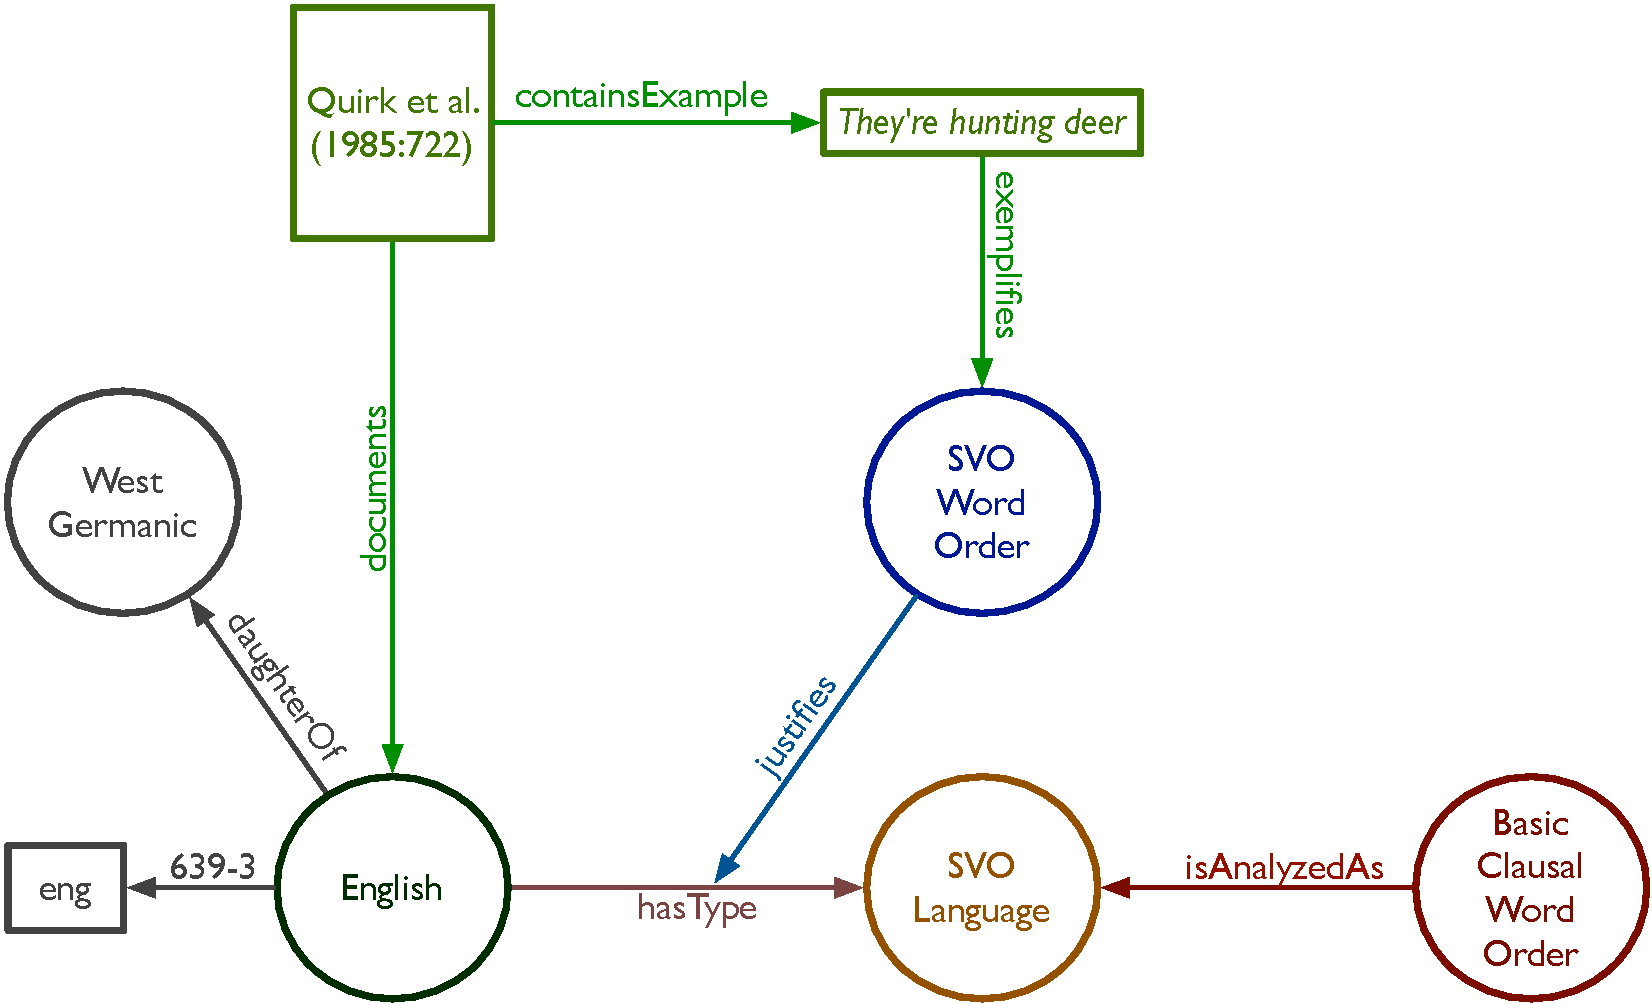
\includegraphics{\imgpath/Indexed.pdf}}
\caption{Adding completeness to a graph-based description \label{MergeIndex}}
\end{figure}

Other elements of completeness could be associated with comparable nodes to what
is seen in \fref{MergeIndex}, though the relationships between the element of
completeness and the descriptive analysis will, of course, not always be as
simple. For instance, if a language showed split word order, this would require
a more elaborate specification in the graph, just as it requires a more
elaborate description in a traditional descriptive grammar. Similarly, if an
element of completeness was associated with a phenomenon not attested in the
language being described, conventions could be adopted to explicitly indicate
its absence, comparable to what is found in the index of
\namecite{Haspelmath:1993Lezgian} (see
\namecite[{\S}2.1]{Good:2004Metadatabase}). Furthermore, just as in a work like
\namecite{ComrieSmith:1977}, where grammatical questions are arranged in a
hierarchy, a full scheme for completeness need not be composed simply of a
``bag'' of questions, but could be specified with additional structure and
information---either using RDF or some other means.

Ultimately, the problem of understanding completeness can be understood as a
kind of data modeling, and better completeness would amount to ``filling out''
more of the elements of an accepted model. For this particular aspect of
descriptive grammars, consensus on the shape of the model itself---whether
digitally encoded or not---appears to be the most difficult issue, with the
technical problems being relatively attenuated.



%%%%%%%%%%%%%%%%%%%%%%%%%%%%%%%%%%%%%%%%%%%%%%%%%%%%%%%%%%%%%
\subsection{Modeling coextensivity\label{ModelingInternal}}
%%%%%%%%%%%%%%%%%%%%%%%%%%%%%%%%%%%%%%%%%%%%%%%%%%%%%%%%%%%%%

Unlike completeness, which must clearly be connected to some community-wide
consensus of what a description should include, coextensivity is
particularized to the documentary record of a language. If the available
documentary information is quite limited, then it might be expected that a
description will be based (more or less) on all of the available data. However,
for languages subject to even a moderate level of investigation, this will often
simply not be possible. Rather, the general goal of the description is not that
it be based on a detailed examination of all of the data. Instead, it
should be based on a sample of the data that results in a description that is
representative of all of the collected data.{\footnote{As will be discussed in
\sref{Coherence}, there are clear connections between coextensivity and
aspects of coherence in descriptive grammars.}}

As mentioned above, there does not appear to have been significant work on how
to measure adequacy of coextensivity. \namecite{Nichols:2005}, however,
considers how much material is needed to produce adequate descriptions
characterized in terms of numbers of words, clauses, and hours, and this would
serve as a good starting point for work on this topic. Ultimately, these
recommendations are probably best considered to be connected to adequacy in
documentation rather than coverage. However, they might serve as proxies for
coextensivity: For instance, her calculation that about 100,000 running
words will allow for ``basic documentation'' suggests that a descriptive grammar
based on a 100,000-word sampling of a much larger corpus is likely to be
sufficient to allow for a reasonable level of analysis of the remaining part of
the corpus by a future investigator, though there will probably still be
significant gaps.

\namecite{Bird:2010} (see also \namecite{Reiman:2010}) describes a documentation
model aimed at under-resourced languages involving the collection of oral texts,
accompanied by oral annotation of a fraction of those texts, and a further
written annotation for a fraction of the orally-annotated texts. While the clear
intention of this process is to provide sufficient annotation (in oral and
written form) of a language to allow the unanalyzed portions to be analyzed in
the future \citep[7]{Bird:2010}, without further research, it seems impossible to
know whether any description creatable on the basis of such a degree of
annotated documentation would actually be sufficient for analyzing the entirety
of the collected materials without the aid of a native speaker. In any event,
the question of what kind of sample of documentary materials can be considered
representative enough to form the basis of a description that would also cover
the remaining materials appears to be an interesting one, and work in this area
would be quite useful for developing general methods for assessing adequacy in
coextensivity.

For transcribed documentary materials, there is at least the possibility of
using a more direct means to assess coextensivity of a description. If a
description can be expressed in a machine-readable form, automated methods could
be employed to apply that description to the entire available dataset (see also
\sref{ConsonanceSec} for related discussion).{\footnote{In principle, these
methods could be applied to untranscribed materials as well if they could
somehow be associated with a reasonable, automatically-derived transcription
using techniques from work on speech recognition. But, of course, that adds a
significant, additional element of complexity.}} The coextensivity of the
machine-readable description could then be considered to be adequate if it can
provide appropriate parses for unanalyzed material. Of course, while some
analytical domains, such as morphological parsing, have seen significant work in
terms of relating traditional documentation to machine-readable parsers (see,
e.g., \namecite{BlackSimons:2008}), most domains of grammar are not yet well
covered. Moreover, while there is at least some relevant work in the domain of
syntax (see \sref{CompatibilitySec}), there seems to be little to no work along
these lines in the domain of phonology (e.g., allowing a user to define a
phoneme inventory and phonotactic constraints and checking to see if
transcriptions are consistent with them).{\footnote{There are, however, tools
that allow one to discover things like phonotactic constraints on the basis of
existing transcriptions, for example Phonology Assistant (see
\namecite{Dingemanse:2008} for a review). Furthermore, the work described
in \namecite{Moran:2012}, though oriented towards typological investigation
rather than description of individual languages, is clearly relevant here.}}

While completeness appears to be representable via data modeling, as discussed
in \sref{ModelingExternal}, this solution does not appear to be applicable to
coextensivity. In particular, the fact that coextensivity is defined in terms of
whatever documentation happens to be available means that it is not amenable to
a treatment involving any kind of general data model. Rather, a more appropriate
approach for modeling coextensivity would appear to be one based on notions from
natural language processing involving the extent to which a parser that has been
``trained'' on a subset of available data can assign correct analyses to data it
has not been trained on (see \namecite{ResnikLin:2010} for overview discussion).\footnote{\namecite{AbneyBird:2010,Bird:2011} offer parallel proposals in
suggesting that one metric for determining whether available documentation is
adequate for capturing the properties of a language is that it is sufficient for
training a machine translation system. } Implementing this kind of approach
generally for digital descriptive grammars is
likely to be quite difficult, however. Creating the relevant kinds of
computational systems, even for well-described languages, is, at this point,
still quite time-consuming and requires resources well-beyond those usually
available to those engaged in language description. Moreover, existing methods are
often heavily reliant on the availability of large quantities of
textual materials, which are simply unavailable for most languages (see also
\namecite{Bird:2011}).




%%%%%%%%%%%%%%%%%%%%%%%%%%%%%%%%%%%%%%%%%%%%%%%%%%%%%%%%%%%%%
\section{Coherence\label{Coherence}}
%%%%%%%%%%%%%%%%%%%%%%%%%%%%%%%%%%%%%%%%%%%%%%%%%%%%%%%%%%%%%

%%%%%%%%%%%%%%%%%%%%%%%%%%%%%%%%%%%%%%%%%%%%%%%%%%%%%%%%%%%%%
\subsection{The components of coherence\label{CoherenceComponents}}
%%%%%%%%%%%%%%%%%%%%%%%%%%%%%%%%%%%%%%%%%%%%%%%%%%%%%%%%%%%%%

A second clear problem with the possibility of taking a distributed approach to
the development of descriptive grammars is that, without specific attention,
they run the risk of becoming incoherent due to distinct conventions and
analyses adopted by different researchers working on pieces of the documentation
or description. Maintaining coherence is, of course, a problem
for all kinds of research, and my goal here will not be to develop the notion
generally, but, rather, to try to specifically model the components of coherence
in descriptive grammars. While the components to be discussed
may not exhaust all of what is required for coherence in
descriptive grammars, those given below appear to represent at least four prominent ones.


\begin{enumerate}%\label{CoherenceList}

	\item{{\bf Consistency in terminology for language-specific categories}: The use
	of terms for language-specific categories is ideally consistently applied
	throughout.}

	\item{{\bf Clarity in terminology for the general audience:} The
	relationships between language-specific categories and comparative concepts
	\citep[in the sense of][]{Haspelmath:Comparative} are ideally made explicit. \label{ClarityP}}
	
	\item{{\bf Consonance of analyses with documentation:} The descriptive
	analyses should ideally be in agreement with what is found in the
	entire documentary record. \label{Consonance}}

	\item{{\bf Compatibility of analyses with each other:} The analyses of
	specific grammatical patterns are ideally compatible with each other
	throughout the description. \label{Compatibility}}

\end{enumerate}

As indicated, the components above represent ideals, and even
single-authored grammars will fail to adhere to them fully. Nevertheless, they
suggest points to pay special attention to if grammatical analysis is to be
distributed since coherence is likely to be an especially problematic area in
this regard.

There are clear connections between certain aspects of coverage and certain
aspects of coherence, at least when these two concepts are understood
informally. This is most clearly seen in relation to coextensivity (see
\sref{TwoCoverages}) and the components of coherence termed \emph{consonance}
and \emph{compatibility} above. Whether or not the coextensivity of a
description would be considered adequate clearly hinges on the extent to which
it is consonant with the documentation and the extent to which all of its
analyses can be brought together into a non-contradictory whole. At the same
time, it seems reasonable to separate these notions. Coextensivity is
intended to reflect the link between available documentation and what
level of description is possible given that documentation, while the
components of coherence are more general than this.
Nevertheless, practically speaking, an important consequence of
the connection between coextensivity and those two components of coherence is
that they may require overlapping technological support.

In the next section, I will discuss how the components of coherence mentioned above could be modeled digitally and discuss existing
technologies that would be relevant for the implementation of those models,
thereby complementing the discussion in \sref{Coverage} and suggesting
additional ways in which the Semantic Web vision might be augmented to
facilitate the creation of digital descriptive grammars in a distributed
fashion. Many of the points to be discussed below should resonate even for those
working on traditional grammatical monographs, but, again, the idea that the
work might be done by many individuals, rather than just one, brings the
relevant issues to the fore. Under such an approach, it will no longer be
obvious who is in charge of the ``quality control'' needed to achieve
coherence, which necessarily prompts us to consider how we might develop means
of ensuring that it is maintained that do not depend on the presence of a
central ``author''.



%%%%%%%%%%%%%%%%%%%%%%%%%%%%%%%%%%%%%%%%%%%%%%%%%%%%%%%%%%%%%
\subsection{Modeling coherence\label{ModelingCoherence}}
%%%%%%%%%%%%%%%%%%%%%%%%%%%%%%%%%%%%%%%%%%%%%%%%%%%%%%%%%%%%%

%%%%%%%%%%%%%%%%%%%%%%%%%%%%%%%%%%%
\subsubsection{Consistency\label{ConsistencySec}}
%%%%%%%%%%%%%%%%%%%%%%%%%%%%%%%%%%%

In discussing \emph{consistency} for the terminology used in a grammatical
description, I refer only to consistency for the terms used to describe the
categories found in the language in question. This dimension of coherence,
therefore, is not intended to apply to the use of terms for general linguistic
concepts, of the sort contained within the GOLD ontology, which I treat as
relevant, instead, to the notion of \emph{clarity}.
The distinction between language-specific categories and general linguistic ones
is not always well-maintained within descriptive grammars, though it is found,
for instance, in \namecite[11]{Haspelmath:1993Lezgian} (on the basis of a
practice employed in \namecite[13]{Comrie:1976}). In that grammar, capitalized
terms are used for language-specific categories and lower-case terms for general
linguistic notions (see \namecite[\S 2.1]{Good:2004Metadatabase}).

Ultimately, the issue of maintaining consistency in a description can, in large
part, be understood as a problem of terminology management (or
\emph{terminography}), which is a distinctive area of research in its own right
(see, e.g., \namecite[1--3]{WrightBudin:1997} and
\namecite[115--159]{Cabre:1999}). Terminology management has some overlap with
lexicography. However, it is primarily oriented with relating concepts to forms,
rather than forms to concepts, as is typical of lexicography
\citep[7--8]{Cabre:1999} (thus making it more comparable to the onomasiological
rather than the semasiological approach to descriptive grammars).

Descriptive linguistics generally already involves a fair amount of informal
terminology management (as evidenced, for instance, by ubiquitous glossing
abbreviation lists and efforts like \namecite{LGR:2008}). Therefore, even if we
did not adopt a distributed approach to the writing of descriptive grammars, the
field could clearly benefit from more robust (and ideally partially automated)
techniques for managing the terms used to describe a given language.
Furthermore, once one considers the possibilities for more distributed
authorship, such techniques would seem to become a necessity in order to
facilitate harmonization of terms across content contributors, whether these are
in Semantic Web form from the start or partial Semantic Web annotation is
attempted for legacy resources. Work of the latter sort could specifically build
on existing research in the area of (semi-)automated term extraction (see
\namecite{AhmadRogers:2001}).

On the whole, technological support for the consistent use of terminology within
a grammatical description appears to be largely underdeveloped. However, it
seems like a potentially profitable area in which to focus efforts in the near
term. This is due to the possibility to make use of existing work on terminology
management in general, as well as on terminological support for the component of
descriptive coherence termed \emph{clarity} here. This latter
area of research will be discussed in the next section, and it can likely serve
as a useful model for the development of tools facilitating consistency in the
use of language-specific terminology, as will be briefly discussed below.



%%%%%%%%%%%%%%%%%%%%%%%%%%%%%%%%%%%
\subsubsection{Clarity\label{Clarity}}
%%%%%%%%%%%%%%%%%%%%%%%%%%%%%%%%%%%

A well-known problem of linguistic description is the use of the same word to
refer to different grammatical concepts or the use of different words to refer
to the same concept across descriptions (see, e.g.,
\namecite[{\S}1]{CysouwEtAl:2005} and \namecite[114]{Zaefferer:2006}). In either
case the potential for confusion is clear, and the issues are especially acute
for work attempting to automate, or partly automate, language comparison on the
basis of digital materials.

This has been one of the key motivations behind the development of the
GOLD ontology
\citep{FarrarLangendoen:2003,FarrarLewis:2007,FarrarLangendoen:2009}, already
discussed in \sref{Context}, which represents the longest-running effort for the
exploitation of Semantic Web technologies for use in descriptive linguistics.
GOLD provides a set of standardized concepts relevant to grammatical description
that can be used to formally define a term used in a language description in
general linguistic terms. For instance, it would allow for the specification
that the English Past Tense verb form expresses a meaning that can be reasonably
related to the general notion of \emph{past tense} specified in GOLD. Of course,
in this case, the terminology is not particularly problematic. However, when
dealing with a form like the Latin Perfect, which would be generally
characterizable as a combination of \emph{perfective} and \emph{past}, rather
than a \emph{perfect} \citep[13]{Comrie:1976}, being able to relate a
language-specific term to more general categories with readily-accessible
definitions, as GOLD allows for, is clearly valuable.

GOLD both provides a standardized termset (with associated URIs for each term)
and structures the members of the termset into an ontology (consisting of a
taxonomy plus some additional information) in order to facilitate automated
processing of linguistic data. Such an ontology is not a strict requirement to
achieve clarity in use of terminology, and a somewhat simpler model is provided
by ISOcat
\citep{KempsSnijdersEtAl:2008:LREC,KempsSnijdersEtAl:2008:ehum}.{\footnote{http://www.isocat.org/}}
ISOcat provides an open registry for data categories relevant
to linguistic resources, allowing an individual linguist or groups of linguists
to publicly register the terms they use and associate them with basic
descriptions of the meaning of the terms. It also provides a unique identifier
for each term which can be used in a Semantic Web context.{\footnote{While
ISOcat's structure does not allow for the specification of an ontology for its
categories, there has been work attempting to develop a degree of ontological
structure around the ISOcat categories in a parallel resource
\citep{WrightEtAl:2010,WindhouwerWright:2012}.}}

ISOcat has a somewhat more ``open'' model than GOLD, insofar as it allows
different groups to register their own categories. By contrast, the addition of
new categories to GOLD is more centrally managed. At the same time, GOLD's
community model explicitly allows for different subcommunities of linguists to
extend the ontology to suit their specific needs (see
\namecite[53--55]{FarrarLewis:2007}). Taken together, an open registration
system like ISOcat in conjunction with tools making it straightforward to
associate an ISOcat category with the appropriate GOLD concepts could provide a
significant degree of support for some of the issues relating to consistency in
the use of terminology discussed above.

There does not yet appear to be significant use of resources like GOLD or ISOcat
to enhance traditional descriptive work. However, due to the efforts that have
been expended on their development, terminological clarity can probably be
considered, at present, the best supported component of coherence discussed
here.




%%%%%%%%%%%%%%%%%%%%%%%%%%%%%%%%%%%
\subsubsection{Consonance\label{ConsonanceSec}}
%%%%%%%%%%%%%%%%%%%%%%%%%%%%%%%%%%%

The development of the documentary paradigm has altered expectations regarding
the extent to which the data on which a description is based should be
accessible. This brings to the fore an issue with respect to coherence which was
always present but was often of little practical significance: To what extent is
a given description, which will often be based on a detailed examination of only
a subset of documentary materials, in agreement with the entire body of
available documentation for a language? Section \ref{ModelingInternal} discussed
related issues from the point of view of ensuring adequate coextensivity.

Because the documentary expectations that have made this problem a practical
concern are relatively new, this issue does not appear to have received
significant attention. The focus, up to the present, has instead been on
developing methods through which a given descriptive claim can be verified on
the basis of supporting documentation in a relatively richly annotated corpus
(see, e.g., \namecite{Thieberger:2009}). But, in the long run, it would also be
ideal if it were possible for sparsely annotated documentation to be
automatically processed on the basis of existing connections between
documentation and description in order to locate possible cases of discord
between the documentation and the description. This processing could involve
such things as, for example, the detection of phonological processes that fail
to apply as expected, the discovery of members of a morphological paradigm which have not been accounted for, or flagging uses of a discourse marker that do not match
its description.

These are, of course, difficult tasks to the extent that they require the
development of sophisticated parsers based on machine-readable grammars---the
descriptive grammatical equivalent of debugging software (see also
\sref{ModelingInternal}). One potentially promising relevant line of work in
this regard involves automated processing techniques that make use of manual
annotation of a fragment of a corpus combined with \emph{active learning} in
which the user provides feedback to an automated system to help improve its
performance. This has been applied to the domain of interlinear glossed text
\citep{BaldridgePalmer:2009,PalmerEtAl:2009,Palmer:2009,PalmerEtAl:2010} and
could, in principle, be applied to other domains as well, reducing the effort
required to create useful parsing tools for a given language. However, the path
from experimenting with these methods to providing robust tools for checking the
complicated relationships involved in consonance between documentary products
(e.g., transcribed texts) and descriptive ones (e.g., a complete grammar based
on those texts) is likely to be a relatively long one. (A different line of
research involving machine-readable grammars, more relevant to the notion of
compatibility, but with potential applications to consonance as well, will be
discussed below.)

An open question in research along these lines is where the most effective
``balancing point'' might be for manual versus automatic annotation and whether
or not even relatively simple types of annotation might facilitate the use of
automated methods in ways that make more effective use of an expert's time. For
instance, it will often be the case that documentary recordings will contain
stretches of different languages, most typically a language of wider
communication and a language being documented. Annotating which stretch is in
which language may be able to be done by someone without special linguistic
expertise on a subset of the recordings to train a machine to do the work across
the whole documentary corpus. This would give an expert linguist a head-start on
more complex kinds of annotation by making it easier for them to locate the most
important stretches of recorded data. The maintenance of consonance in the
relationship between documentary products and derivative descriptive ones would,
thereby, be facilitated. Such a scenario suggests the possibility that taking
full advantage of a more distributed approach to grammatical description may
require us to consider crafting non-prototypical documentary products---in this
case a very sparse kind of linguistic annotation.{\footnote{This scenario also
recalls recent work, such as \namecite{SnowEtAl:2008}, which suggests that
internet marketplaces where workers can be recruited to perform relatively
simple annotation tasks at much lower rates than individuals with linguistic
training may be useful for language research. However, see
\namecite{FortEtAl:2011} for discussion of ethical complications potentially
associated with using such marketplaces, related to the limited rights and wages
typically granted to workers.}}




%%%%%%%%%%%%%%%%%%%%%%%%%%%%%%%%%%%
\subsubsection{Compatibility\label{CompatibilitySec}}
%%%%%%%%%%%%%%%%%%%%%%%%%%%%%%%%%%%

The final dimension of coherence to be discussed here, compatibility, has
already seen some attention in the computational linguistics literature in the
area of grammar engineering, which seeks to create machine-readable versions of
formal grammars (see, e.g., \namecite{Bender:2008}). Among other things, these
grammars allow linguists to automatically test the extent to which their
analysis of a given phenomenon interacts with other analyses as expected,
something which is more or less impossible to do by hand.{\footnote{Grammar
engineering can also play a role in maintaining consonance, insofar as it can help locate instances of data that
cannot be analyzed at all by a given formal grammar, suggesting gaps in a
description.}} Moreover, there have been efforts to ensure that grammar
engineering work done for better-resourced languages can be used to facilitate
the development of machine-readable grammars for lesser-resourced languages
\citep{BenderEtAl:2010}, addressing an issue raised at the end of
\sref{ModelingInternal} in the discussion of coextensivity. Such tools can even
potentially play a role in helping linguists choose among competing descriptive
hypotheses \citep{Bender:2010}.

\namecite{Bender:2008:Wambaya} reports the results of work which made use of a
general grammar engineering system to create a machine-readable grammar for a
language typologically quite distinct from those languages that have informed
most computational research. Strikingly, it was possible to create a reasonable
new machine-readable grammar for this language in a timeframe of about six
weeks. This is, of course, only a small fraction of the time it takes to write a
traditional descriptive grammar. It suggests that work in grammar engineering
has reached a point where relatively limited collaborations between linguists
specializing in this area and those working on underdescribed languages may
yield worthwhile results for language description with respect to ensuring
compatibility among analyses. More generally, this work provides a model for how
to move forward in the development of computational techniques to facilitate the
creation of digital descriptive grammars: Lessons learned from the development
of computational tools for better-resourced languages, often at great cost, can
ultimately be applied to lesser-resourced languages at much lower cost (see also
\citet{Bendertv}).

The work described above is primarily focused on syntactic phenomena. Comparable
tools exist for some aspects of morphophonological analysis (see, e.g.,
\citet{BlackSimons:2008} and \citet{Maxwelltv}), though there has not yet been much work on
integrating tools from each of these domains (though see
\namecite{BenderGood:2008} for some discussion of possibilities). Furthermore,
other domains of grammar do not appear to be well-supported yet at all, with
phonology standing out as an area where the lack of obvious tools does not seem
to present major technical problems but, rather, results from a lack of
dedicated effort (though see \namecite{Moran:2012}). For example, a tool allowing a linguist to specify phonotactic
constraints and ensure their overall compatibility would appear to be much more
straightforward to develop than the already existing tools supporting syntactic
analysis mentioned above. Nevertheless, to the best of my knowledge no such tool
exists. (See also \sref{ModelingInternal}.) In other domains, like semantics and
pragmatics, the tool gap is less surprising given the difficulties of conducting
even informal descriptive work in these areas.

While the discussion here has been primarily in terms of issues regarding
parsing language data, some computational systems are designed to be
bidirectional, both parsing and generating language data (see
\namecite[6]{BenderLangendoen:2010} for discussion relevant in the present
context). While I am not aware of specific proposals in this regard, the ability
of such systems to generate data has potential applications for testing
compatibility (as well as consonance) of grammatical analyses adopting
onomasiological approaches. This would require a machine-readable means to
describe the relevant ``functions'' which would serve as an input for the
generation of predicted forms in a given language. The generated forms could be
compared against attested forms to gauge the extent to which they match each
other.



%%%%%%%%%%%%%%%%%%%%%%%%%%%%%%%%%%%%%%%%%%%%%%%%%%%%%%%%%%%%%%%%%%%%%%%%%%%%%%%%
\section{Conclusion\label{Conclusion}}
%%%%%%%%%%%%%%%%%%%%%%%%%%%%%%%%%%%%%%%%%%%%%%%%%%%%%%%%%%%%%%%%%%%%%%%%%%%%%%%%

%%%%%%%%%%%%%%%%%%%%%%%%%%%%%%%%%%%%%%%%%%%%%%%%%%%%%%%%%%%%%
\subsection{Building on existing infrastructure}
%%%%%%%%%%%%%%%%%%%%%%%%%%%%%%%%%%%%%%%%%%%%%%%%%%%%%%%%%%%%%

Overall, we have seen above that, if we take the distributed model of research
implied by Semantic Web technologies seriously, we are presented with the
problem of losing desirable characteristics of traditional resources not
embedded within the design of the Semantic Web itself. However, with appropriate
conceptual models of key components of a traditional resource, we can devise
explicit characterizations of what we have lost which allow us to see how we can
augment the Semantic Web (or any comparable endeavor) in ways that reincorporate
the ``missing'' features into our new kinds of resources.

In focusing on coverage and coherence, the overall vision that emanates from
this discussion is one where Semantic Web technologies would form a basic
infrastructure to express statements in ways that make them straightforwardly
registrable and reusable, but where the set of statements comprising a
grammatical description would be subject to additional data processing and
validation. This would involve techniques ranging from the development of formal
data models (to help verify completeness), to the deployment of tools for
terminology management (to help ensure consistency), to the use of
machine-readable formal grammars (to help test for compatibility).

At the same time, significant areas have been identified where tool support or
appropriate models of practice are lacking, though a path to developing those
tools or models can be outlined. This was seen, for instance, in the domain of
coextensivity, where there has been relatively little research on determining
what an appropriate documentary ``sample'' might look like. It was also seen in
the domain of consonance where tools for verifying that nowhere in the
documentation is a description contradicted have not received serious attention on
either the conceptual or implementation side. In both cases, methods from
natural language processing were put forth as presenting possible solutions to
these problems.

Nevertheless, a significant result, I believe, of this survey is the extent to
which many existing technologies provide models (if not necessarily
``off-the-shelf'' tools) for how we might go about developing a tool ``ecology''
(see \namecite{Good:ToolEcology}) for distributed grammatical description with
less effort than might appear to be needed at first. Importantly, even if a
given tool type requires re-implementation to be usable in a documentary and
descriptive context, modeling a new tool on an existing one is likely to save
considerable time and resources, when set against developing it completely anew.



%%%%%%%%%%%%%%%%%%%%%%%%%%%%%%%%%%%%%%%%%%%%%%%%%%%%%%%%%%%%%%%%%%%%%%%%%%%%%%%%
\subsection{Deconstructing \emph{our} problems\label{Deconstructing}}
%%%%%%%%%%%%%%%%%%%%%%%%%%%%%%%%%%%%%%%%%%%%%%%%%%%%%%%%%%%%%%%%%%%%%%%%%%%%%%%%

To conclude, this has paper has been intended to be an exercise in what one
might call ``theoretical'' electronic grammaticography (though grounding the
discussion in specific relevant technologies). While its starting point (see
\sref{Context}) was a technical discussion of the Semantic Web, ultimately its
specific technical details were of less importance than the model that it
provided for a more distributed approach to data dissemination and curation,
which has clear potential applications for many areas of scholarship, but
especially descriptive grammars. This is due to their complexity in terms of the
relationship of descriptive claims to documentation, the breadth of their
subject matter, and the interconnectedness of the elements of description.

While the discussion here has been framed as one where the distribution of the
work of describing a language is dispersed across multiple contributors, the
long-term nature of most descriptive work also means that it is distributed
across time, even if there is only a single main creator. Because of this, many
of the models and techniques described here would certainly also be of value in
cases where effort is expended primarily by one person, but over a long enough
period that they may find it difficult to keep track of their own progress.

Two particular issues were the focus here, coverage and coherence. These are
undoubtedly important aspects of traditional descriptive grammars. However, it
should be emphasized that they are far from the whole story. For instance, one
of the criteria listed by \namecite[396]{Rice:2006:Grammars} as an aspect to
writing an effective grammar is ``richness of illustration'', a clearly
important concern not considered here at all.

Moreover, the framework introduced here does not allow for the expression, in
any straightforward way, of the idea that languages have a basic ``plan'' or
structural ``genius'', to borrow from the famous formulation of
\citep[127]{Sapir:1921}. This idea has been reflected in the intuitions of both
formal and descriptive linguists (see, e.g., \namecite[6--9]{Baker:1996} and
\namecite[3--4]{EvansDench:2006}). However, it is difficult to imagine how it
could be expressed in the deliberately reductionist framework of the Semantic
Web, making it clear that we should not understand a reconceptualization process
like the one offered here as a means of replacing our traditional understanding
of what makes a descriptive grammar ``good''. Rather, it should be seen as an
exercise in understanding how we can use technology to enhance what we already
know to be good (see also \namecite[42--43]{DobrinEtAl:2009}).

Ultimately, the goal of a study like this one is not to set our agenda on the
basis of what a given technology offers but, rather, to clarify which existing
technologies can fulfill our needs and to map out plans for the creation of new
technologies. The Semantic Web may have prompted consideration of many of the
ideas discussed here, but it cannot serve as a substitute for crafting a vision
for the future of linguistic resources with our own values serving as its
foundation.



% \psmall
% 
% \hfill Jeff Good
% 
% \hfill jcgood@buffalo.edu
